\section{Ziel}
In diesem Versuch sollen mithilfe von Neutronen verschiedene Proben aus Vanadium und Silber
 Radioaktiv aktiviert werden.
Von den erzeugten radioaktiven Isotopen dieser Proben wird anschließen die Halbwertszeit ermittelt.

\section[Theoretische Grundlagen]{Theoretische Grundlagen\footnote[1]{Unter Verwendung von \cite[]{man:v702}}.}


\subsection{Anregung der Proben}

\noindent
In diesem Versuch werden drei Radioaktive Isotope aus in der Natur stabilen Metallen erzeugt.
\begin{align}
    \ce{^{51}V}, & \ce{^{107}Ag},  \ce{^{109}Ag}
\end{align}

Dies wird erreicht in dem das Verhältnis von Neutronen und Protonen in den Kernen des Elements verändert wird.
Hierzu werden sich Kernreaktionen mit Neutronen zunutze gemacht.
Eine Kernreaktion eines Atomkerns A mit einem Neutron beginnt mit der Absorption des Neutrons im Atomkern.
Den neuen so entstandenen angeregten Kern A* nennt man Zwischenkern oder Compoundkern.
Er ist durch die Bindungsenergie des Neutrons auf einem höheren Energielevel als der einfache Atomkern.
Diese Energie verteilt sich auf die gesamten Nukleonen, weshalb die Energie des Atomkerns meist nicht mehr ausreicht
um das ganze Nukleon wieder abzustoßen.
Das ist vor allem der Fall wenn die Neutronen eine geringe Geschwindigkeit haben.
Stattdessen wird die Energie in Form eines $\gamma$-Quants emittiert wonach das Atom wieder in einem nicht angeregten Zustand befindet.
Es läuft folgende Reaktion ab:
\begin{align*}
    \ce{^{m}_{z}A} + \ce{^{1}_{0}n} \rightarrow \ce{^{m+1}_{z}A*} \rightarrow \ce{^{m+1}_{z} A} + \gamma .
\end{align*}
Dieser neu entstandene Kern $\ce{^{m+1}_{z} A}$ ist oft nicht stabil, weil er mehr Neutronen enthält
als er in einem stabilen Zustand haben kann.
Er wandelt in einem $\beta^{-}$-Zerfall in ein Neutron in ein Proton um und emittiert 
Elektron $\beta^{-}$ und Antineutrino $\overline{\nu}_\text{e}$ mit einer Kinetischen Energie $E_\text{kin}$:
\begin{align*}
    \ce{^{m+1}_{z} A} \rightarrow \ce{^{m+1}_{z+1} C} + \beta^{-} + E_\text{kin} + \overline{\nu}_\text{e}
\end{align*}

\noindent
In diesem Versuch werden die folgende Kernreaktionen gemessen:
\begin{align*}
    \ce{^{51}_{23} V}   \rightarrow \ce{^{52}_{23} V}   \rightarrow \ce{^{52}_{24} Cr}  + \beta^{-} + E_\text{kin} + \overline{\nu}_\text{e}  \\
    \ce{^{107}_{47} Ag} \rightarrow \ce{^{108}_{47} Ag} \rightarrow \ce{^{108}_{48} Cd} + \beta^{-} + E_\text{kin} + \overline{\nu}_\text{e}  \\
    \ce{^{109}_{47} Ag} \rightarrow \ce{^{110}_{47} Ag} \rightarrow \ce{^{110}_{48} Cd} + \beta^{-} + E_\text{kin} + \overline{\nu}_\text{e}  \\
\end{align*}


\subsection{Wirkungsquerschnitt}
\label{sec:teo_wirkungsquerschnitt}
Der Wirkungsquerschnitt $\sigma$ ist eine geometrische Überlegung, 
um die Wahrscheinlichkeit von Kernreaktionen darzustellen.
Wenn $n$ Neutronen, die auf eine dünne Folie mit der Dicke d [\unit{\cm}] und der Dichte 
K[ Atome/\unit{\cm\cubed}] geschossen werden, wobei $u$ Einfänge auftreten, dann ergibt sich
der Wirkungsquerschnitt mit
\begin{align*}
    \sigma = \frac{u}{n K d}
\end{align*}
Eine Vorstellung des Wirkungsquerschnitts ist die einer Zielscheibe.
Die Neutronen treffen die Kerne, die einen gewissen Anteil der Fläche mit ihren
Querschnitten abdecken.
Der Querschnitt eines Kerns ist in der Größenordnung von \qty{10e-24}{\cm\squared}.
Diese Klassische Vorstellung von Atomkernen die einen Querschnitt haben und von Neutronen
getroffen werden können, ist tatsächlich weiterführend, wenn die De-Broglie Wellenlänge
der Neutronen $\lambda = h/m_n v$ klein im Vergleich zum Kernradius R($\simeq \qty{10e-12}{\cm}$) ist.
(Hier ist $h$ das Plancksche Wirkungsquantum und $m_n$ die Neutronenmasse)
Für Wellenlängen, die  $\leq$ R sind treten Streuungseffekte an den Kernen auf.
In Experimenten werden Wirkungsquerschnitte beobachtet, die um mehrere Zehnerpotenzen größer als die
als in der geometrischen Rechnung. 
Mit der Quantenmechanik können bestimmte Energieniveaus identifiziert werden, bei denen
die Neutronen besonders gut absorbiert werden können.
Breit und Wigner haben eine Formel angegeben, 
die den Wirkungsquerschnitt als Funktion der Neutronenenergie E darstellt:
\begin{align*}
    \sigma(E) = \sigma_0 \sqrt{\frac{E_{r_i}}{E}} \frac{\tilde{c}}{\left(E - E_{r_i} \right)^2  +  \tilde{c}}
\end{align*}
$\tilde{c}$ und $\sigma_0$ sind charakteristische Konstanten der Kernreaktion.
Für kleine Energien $E<< E_{r_i}$ kann $\left(E - E_{r_i} \right)^2$ als konstant angenommen werden.
Dafür gilt also
\begin{align*}
    \sigma ~ 1/ \sqrt{E} ~ 1/v . 
\end{align*}
Für niedrigere Geschwindigkeiten gibt es also höhere Einfangswahrscheinlichkeiten des Neutrons

\subsection{Erzeugung niederenergetischer Neutronen}
Um eine möglichst effiziente Anregung zu erreichen werden also 
langsame Neutronen gebraucht.
Zunächst werden die Neutronen durch Beschuss von Beryllium Kernen mit 
$\alpha$-Teilchen freigesetzt:
\begin{align*}
    \ce{^{9}_{4}Be} + ^{4}_{2}\alpha \rightarrow \ce{^{12}_{6}C} + \ce{_{0}^{1}n}
\end{align*}
Die $\alpha$-Teilchen stammen aus dem Zerfall von $\ce{^{226}Ra}$-Kernen. 
Die Neutronen haben Energien von bis zu $\qty{13.7}{\mega\eV}$. 
Um die Energie der Neutronen zu vermindern werden sich elastische Stöße zunutze gemacht
Der Maximale Energieübertrag bei einem Elastischen Stoß beträgt
\begin{align*}
    E_\text{ü} = E_0 \frac{4Mm}{\left(M + m\right)^2}
\end{align*}
Den besten Energieübertrag gibt es demnach bei gleichschweren Stoßpartnern.
Hierfür bietet sich Wasserstoff an, da es aus nur einem Proton besteht, welches in etwa
gleich scher wie ein Neutron ist. 
Die Neutronenquelle befindet sich also in einem Mantel aus Paraffin (siehe Abb. \ref{fig:neutronenquelle}).
Durch Mehrfache Stöße eines Neutrons mit den Protonen des Paraffin erreichen sie eine
Energie, die der mittleren kinetischen Energie der Moleküle bei Raumtemperatur angenähert ist.
Diese Energie liegt bei etwa \qty{0.025}{\eV} für T = \qty{290}{\kelvin}.
\begin{figure}
    \centering
    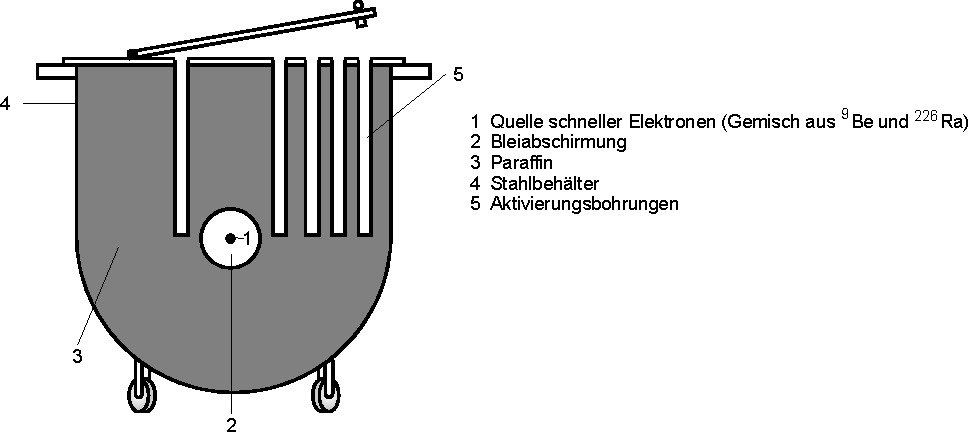
\includegraphics{Abbildungen/Neutronenquelle.pdf}
    \caption{Querschnitt durch die heir verwendete Quelle von Neutronen \cite[vgl.]{man:v702}}
    \label{fig:neutronenquelle}
\end{figure}



\subsection{Halbwertszeit}
\label{sec:teo_halbwertszeit}
Die Halbwertszeit eines radioaktiven Materials ist ein statistischer Wert,
der bei einer großen Anzahl an Teilchen die Zeit bestimmt, bis die Hälfte der Teilchen zerfallen ist.
Die Zahl der Noch nicht zerfallenen Kerne in einer Probe wird durch 
\begin{align}
    N(t)= N_0 e^{-\lambda t}
\end{align}
beschrieben.
Die Halbwertszeit $T$ der Probe ergibt sich damit aus
\begin{align}
    1/2 N_0 = N_0 e^{-\lambda T} \Leftrightarrow T = \ln(2)/\lambda
    \label{eq:T_aus_lambda}
\end{align}
Um die Halbwertszeit aus den gemessenen Zerfällen in einem Zeitintervall $\Delta t$
zu ermitteln werden sich die Eigenschaften der e-Funktion zunutze gemacht.
Es gilt
\begin{align}
    \ln N_{\Delta t} = \ln{N_0 (1- e^{-\lambda \Delta t})} - \lambda t
    \label{eq:lambda_aus_N}
\end{align}
Der Wert für $\lambda$ ergibt sich aus einer linearen Ausgleichsrechnung, da
\begin{align*}
    \ln{N_0 (1- e^{-\lambda \Delta t})} = \text{const.}
\end{align*}

\noindent
Die Länge des Zeitintervalls $\Delta t$ muss sorgfältig gewählt werden und ist vom
zerfallenden Isotop abhängig.
Bei zu klein gewähltem $\Delta t$ sind die statistischen Schwankungen zu groß um
einen erkennbaren Effekt zu erhalten. 
Bei zu groß gewähltem $\Delta t$, etwa in der Größe der Halbwertszeit T 
gibt es nicht mehr genug Datenpunkte um eine zielführende Ausgleichsrechnung zu machen.



\subsubsection{Halbwertszeit bei zwei Silberisotopen}
Bei dem Zerfall der angeregten Silberprobe ist zu beachten, dass die Probe in etwas zu 
gleichen Teilen zwei verschiedene Isotope enthält.
Die Halbwertszeit dieser Isotope ist nur feststellbar, weil die Halbwertszeit des einen
des $\ce{^{108}Ag}$ Isotops deutlich länger als die Halbwertszeit von $\ce{^{110}Ag}$ ist.
Im Halblogarithmischen Diagramm folgt die Zerfallszahl ab einer gewissen Zeit $t^{*}$ einer Gerade.
Bei dieser Gerade ist nur noch der langlebigere Zerfall aktiv.
Mit der Ausgleichsrechnung aus Abschnitt \ref{sec:teo_halbwertszeit} 
lässt sich der Koeffizient $\lambda_{l}$ für die Zerfallsfunktion dieses Isotops herleiten.
Für den Koeffizienten $\lambda_{k}$ des kurzlebigeren Isotops
wird die Zerfallsfunktion für die Werte $t > t^*$ an den Stellen $t_i < t_\text{max} < t^*$ von den
Werten an diesen Stellen abgezogen. 
Daraus ergibt sich dann die Ausgleichsrechnung für das Kurzlebigere Isotop.
In Abbildung \ref{fig:teo_e-funktionen-krampf} wird das Ergebnis dieser 
Rechnung auf einer Logarithmischen Skala dargestellt.

\begin{figure}
    \centering
    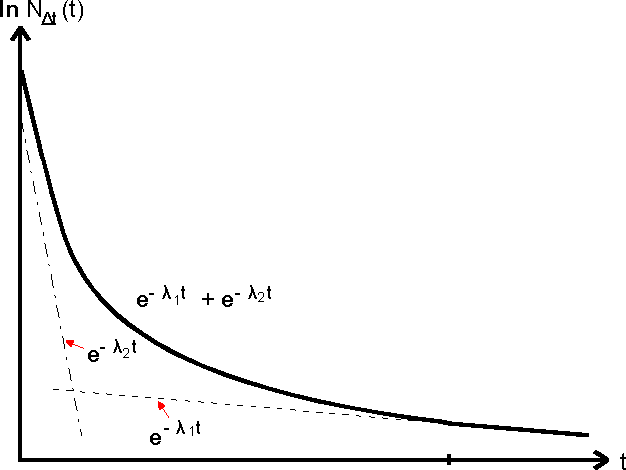
\includegraphics{Abbildungen/Zerfallskurven.pdf}
    \caption{Überlagerung der Zerfallskurven für die Silber Isotope. \cite[vgl.]{man:v702}}
    \label{fig:teo_e-funktionen-krampf}
\end{figure}


%%% To Do
% Wirkungsquerschnitt für schnelle und langsame Neutronen
% Erzeugung Niederenergetischer Neutronen